% !TEX root = ../thesis.tex

% Tässä osassa esitetään tulokset ja vastataan tutkielman alussa
% esitettyihin tutkimuskysymyksiin. Tieteellisen kirjoitelman
% arvo mitataan tässä osassa esitettyjen tulosten perusteella.

% You have done your work, but that’s1 not enough.
% You also need to evaluate how well your implementation works. The
% nature of the evaluation depends on your problem, your method, and your
% implementation that are all described in the thesis before this chapter. If
% you have created a program for exact-text matching, then you measure how
% long it takes for your implementation to search for different patterns, and
% compare it against the implementation that was used before. If you have
% designed a process for managing software projects, you perhaps interview
% people working with a waterfall-style management process, have them adapt
% your management process, and interview them again after they have worked
% with your process for some time. See what’s changed.
% The important thing is that you can evaluate your success somehow.
% Remember that you do not have to succeed in making something spectacular;
% a total implementation failure may still give grounds for a very good master’s
% thesis—if you can analyze what went wrong and what should have been done.

\documentclass[thesis.tex]{subfiles}

\begin{document}

\chapter{Experiment}
\label{chapter:experiment}

The purpose of the experiment was to investigate the feasibility and performance (precision) of photoluminescence-based product authentication using the fingerprint method described in the previous chapter. Additionally, another set of results was computed by replacing the fingerprint analysis and matching steps with a more computationally intensive histogram-based approach, which is discussed briefly in more detail in Chapter \ref{chapter:results}. The following Chapter \ref{chapter:setup} introduces the luminophores, the hardware and the various capture, analysis and matching parameters used in the experiment. The results for both the fingerprint and the histogram method are summarized and compared in Chapter \ref{chapter:results}. Finally, some artefacts introduced by the capture pipeline are presented.

\section{Setup}
\label{chapter:setup}

The luminophores used in the experiment were LumiNova\textregistered\ red (O), green (G) and blue (DB) pigments. Each of the pigments was mixed with a transparent carrier to form a stock solution. The stock solutions were pipeted in increments of $50\mu l$ onto white blank cartons to form eight unique taggants. Two samples ($a$ and a replicate sample $b$) were taken from each solution, so a total of 16 different taggants were prepared for the experiment. The taggants and the amount of phosphor and transparent carrier used to create them are listed in Appendix \ref{appendix:taggants}. For information about the chemical properties of the LumiNova\textregistered\ pigments the reader is referred to \cite{luminova}.

The taggants were captured using Samsung S4 (version 4.4.2) and Lumia 1020 (version WP8.1) smartphones. The MFD of the S4 and the 1020 was determined empirically to be around 100mm and 150mm, respectively. The height of the camera module was adjusted accordingly to ensure that no image blur would be introduced. As depicted in Figure \ref{figure:camera_module} the light source was positioned perpendicular to the taggant as per the common conventions in fluorescense spectoscopy \cite{spectroscopy-principles}. Yongnuo YN565EX\footnote{Yongnuo YN565EX User Manual: \url{http://www.yongnuo.com.cn/usermanual/pdf/USER_MANUAL_YN565EX_EN.pdf}} external camera flash was used as the light source as it provided a convenient way to produce a high quality, full-spectrum white light for the photoexcitation. The power and zoom level of the flash were set to 1/32 and 24mm, respectively. The zoom level of the flash was set to the widest supported level assuming that the taggant would be more suspectible to uneven exposure on higher levels of zoom due to a more concentrated burst of light. The power level of 1/32 was selected by observing at which level the captured frames would no longer be overexposed.

The taggants were captured in a dimly lit room to minimize interference of ambient light. In total, nine different capture presets were defined: six presets for the Samsung S4 ($an$) and three presets for the Lumia 1020 ($wp$). The capture presets and the corresponding parameter values are listed in Appendix \ref{appendix:capture-presets}. The parameter values are discussed more thoroughly in Chapter \ref{chapter:discussion}. All of the 16 taggants were captured with each of the presets resulting in a corpus of 144 fingerprints (including $a$ and $b$ samples). The fingerprints were labeled based on the capture preset and the taggant in the following format: \emph{\{preset\}/\{taggant\}\{sample\}} (e.g. \emph{wp200/Sa}). The taggants captured with the Samsung S4 and Lumia 1020 are presented in Figure \ref{figure:taggants} for preview.

\begin{figure}[h]
\label{figure:taggants}
\centering 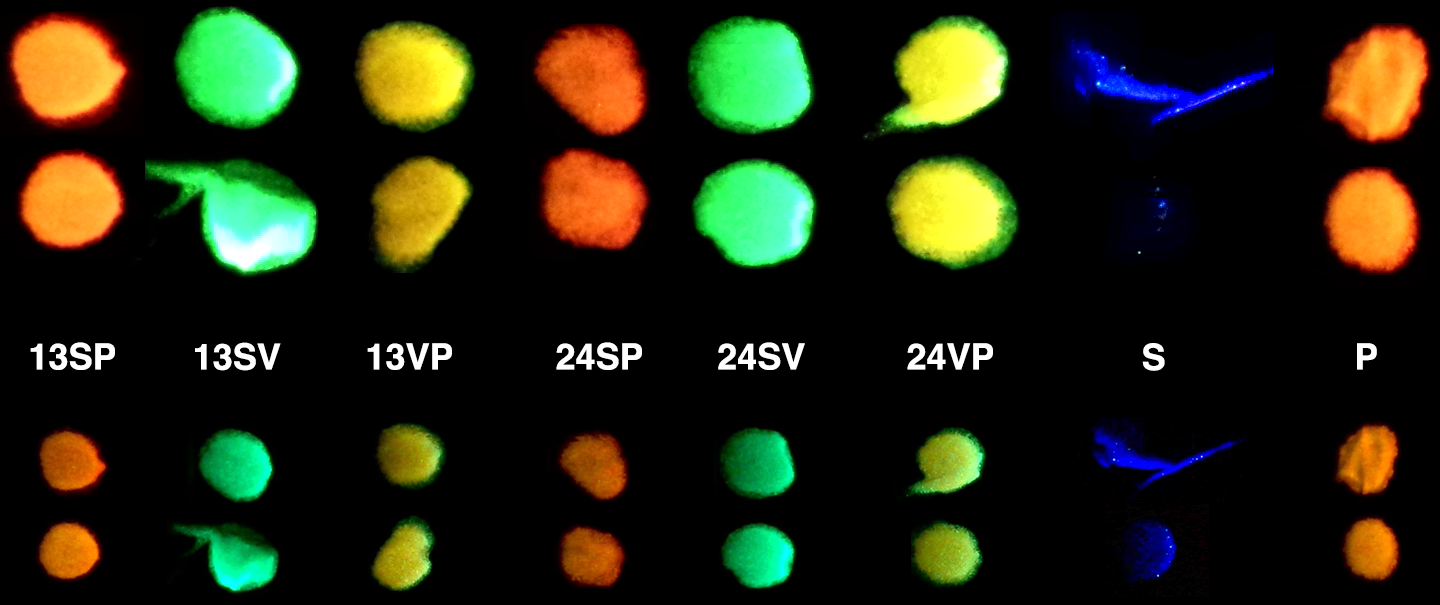
\includegraphics[width=\textwidth,height=\textheight,keepaspectratio=true]{images/experiment/taggants}
\caption{Captured taggant samples \emph{a} (upper) and \emph{b} (lower) for both the Samsung S4 (top two rows) and the Lumia 1020 (bottom two rows).}
\end{figure}

After capture, each taggant was given 15 minutes to reset to ground state in order to minimize the effect of residual afterglow on subsequent captures. The taggants were also protected from any external sources of light before the experiment to prevent exciting the luminophore prior to capture and introduce bias.

\section{Results}
\label{chapter:results}

The performance of the fingerprint pipeline was evaluated by computing the similarity score of each fingerprint against the rest of the corpus. The fingerprint's countersample (sample \emph{a} or \emph{b}) was expected to receive the lowest score (best). For example, for fingerprint \emph{an200/24SPa} the closest match was expected to be \emph{an200/24SPb}. For fingerprints captured with the Samsung S4 the resolution variant and its countersample were also considered a match. That is, for \emph{an200/24SPa} valid matches would include three fingerprints: \emph{an200/24SPb}, \emph{an200r/24SPa} and \emph{an200r/24SPb}. For brevity, valid matches of a fingerprint are henceforth referred to as \emph{sibling fingerprints}.

The similarities were computed using the fingerprint matching algorithm presented in Chapter \ref{chapter:fingerprint-matching} and a more computationally intensive histogram-based method, which could also be used to assess the performance of the fingerprint matching algorithm. The histogram method was implemented using the \emph{compareHist()} function of OpenCV's image processing API to compute the \emph{Hellinger distance} between two histograms. As input the function was given the Hue-Saturation histograms of the frames of two fingerprints \emph{A} and \emph{B} frame-by-frame. The sum of the computed Hellinger distances denoted the similarity between the two fingerprints -- the lower sum, the better a match. Hellinger distance was chosen as the comparison method as it is considered a de facto approach for comparing probability distributions (e.g. histograms) \cite{hellinger}. To avoid ambiguity the fingerprint analysis and matching process and the histogram-based approach are henceforth referred to as \emph{fingerprint and histogram methods}. The method parameter values used in the experiment are summarized in Appendix \ref{appendix:method-parameters}.

For both methods the computed similarity scores were consolidated into a $n\times n$ similarity matrix, where $n$ was equal to the number of fingerprints in the corpus (144) and each row/column represented the similarity of a fingerprint to the rest of the corpus. The resulting matrix would thus be a \emph{zero-diagonal symmetric matrix}. The similarity matrices were first used for finding fingerprint clusters. The clusters would indicate -- on a broad level -- how accurate the given method was. Ideally, the clustering would produce 48-72 clusters (one for each group of sibling fingerprints) each consisting of 2-4 sibling fingerprints. The results of the clustering are visualized in Figure \ref{figure:clusters}. Each bar in the graphic represents a fingerprint, where the color denotes the taggant and height the interval duration. That is, the clusters would ideally be of equal color and height -- a group of sibling fingerprints. It should be noted that the visualization distinguishes presets only by the difference in the interval duration. Thus, for example the platform a given fingerprint was captured under (Android/Windows Phone) is not communicated by the visualization.

\begin{figure}[h]
\label{figure:clusters}
\centering 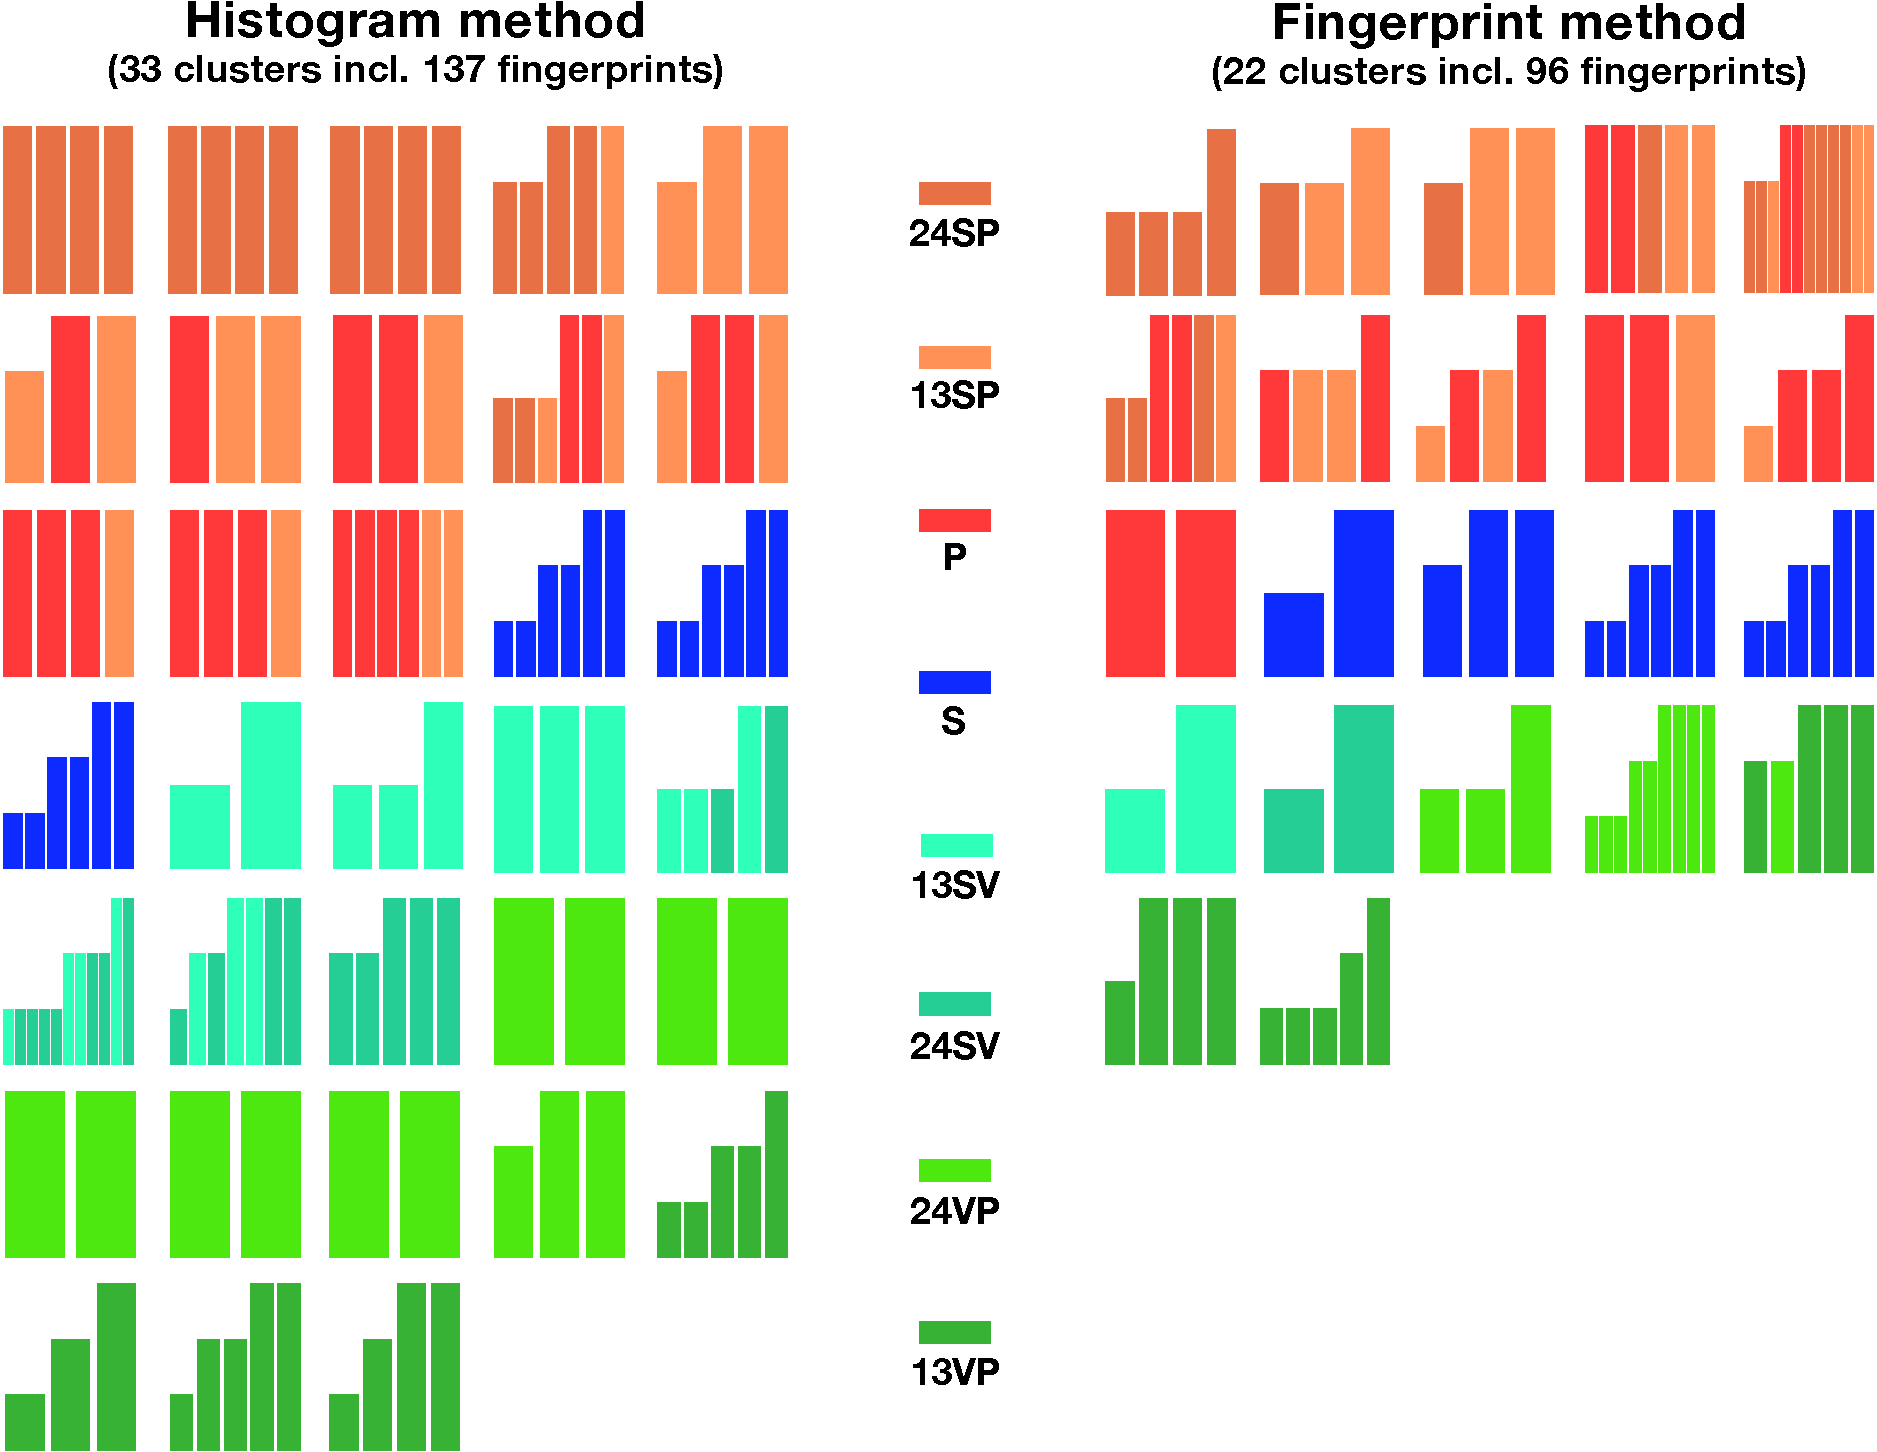
\includegraphics[page=1,width=\textwidth,height=\textheight,keepaspectratio=true]{images/experiment/clusters}
\caption{Fingerprint clusters based on the similarities computed by the histogram and fingerprint methods. Each bar represents a fingerprint, where the color denotes the taggant and height the interval duration.}
\end{figure}

The fingerprints were clustered using affinity propagation (AP) and its implementation in R\footnote{\url{http://cran.at.r-project.org/web/packages/apcluster}}. The benefit of AP clustering is that no apriori knowledge of the number of clusters to be computed is required. It is best suited for small to medium-sized datasets as it is computationally heavier than most other clustering algorithms. The similarity matrices were processed by the algorithm using the default values for all parameters except for the \emph{q} parameter (sample quantile threshold), which was set to $q=0.95$. The sample quantile threshold ($0-1$) can be used to adjust how aggressively the algorithm clusters the data -- the higher the value, the more clusters the algorithm tries to find. For further information about AP clustering and its R implementation the reader is referred to \cite{affinity_propagation}.

To gain more insight into
- comparison vs. histogram approach
- Margin 10, 15 and 25\% to indicate histogram > fingerprint method (=> focus on histogram method)
  - - boundary conditions (max margin and max count)

\begin{figure}[h]
\centering 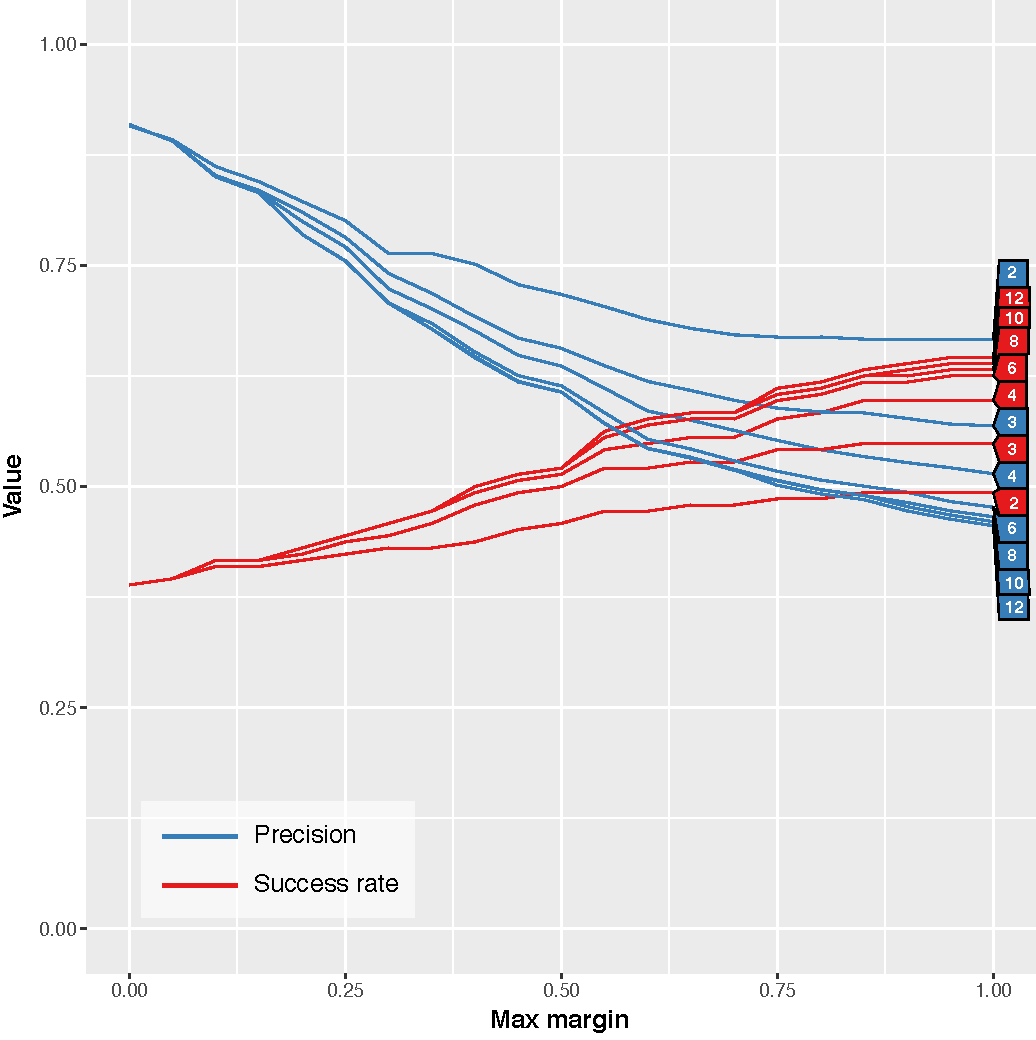
\includegraphics[page=1,width=\textwidth,height=\textheight,keepaspectratio=true]{images/experiment/match_precision}
\end{figure}
\begin{figure}[h]
\centering \includegraphics[page=2,width=\textwidth,height=\textheight,keepaspectratio=true]{images/experiment/match_precision}
\end{figure}
\begin{figure}[h]
\centering \includegraphics[page=3,width=\textwidth,height=\textheight,keepaspectratio=true]{images/experiment/match_precision}
\end{figure}
\begin{figure}[h]

- Evaluate the effect of capture (/analysis) params
  - ignore resolution, look at interval?
  - find anomalies
  - visualize which taggants perform the best, and why? (good match: an\_600/24SPa, an\_600\_r/24VPb)

\centering \includegraphics[page=7,width=\textwidth,height=\textheight,keepaspectratio=true]{images/experiment/tags_configs}
\end{figure}

- present artefacts


\end{document}